%!TEX root = main.tex
\chapter{Implementation}
\label{chap:implementation}
% In many cases, you will not be able to realize the full design. Often the implementation is only a demonstrator of ideas. 
% It is therefore important that you focus on the most important aspects of your system (depending on research questions). 
% In the report you have to justify the choices that are done.
This chapter described the PeacefulBanana architecture, the technology we used to implement it and the functionality it provides. 
We will elaborate on the decisions made in order to develop the PeacefulBanana tool, and the rationale behind the decisions made connected with the Mirror CSRL cycle model described in section \ref{mirrorsection}. 

\section{Application Architecture}
Figure \ref{ClientServerGithub} shows an overview of the system design and the interaction between users, the web-server and GitHub. Each PeacefulBanana user visits the web-application through a web-browser. PeacefulBanana runs on a dedicated server and is able to serve many users at the same time. In the background the PeacefulBanana application communicates with GitHub through the GitHub API(see Section \ref{githubapi}) and synchronizes project and user-data in real time while users perform their tasks. Users connect their local PeacefulBanana account with their GitHub account in order to gain access to projects. All data collected from GitHub is stored locally on the server in a database(See section \ref{sec:database}). 
\begin{figure}[H]
    \centering
        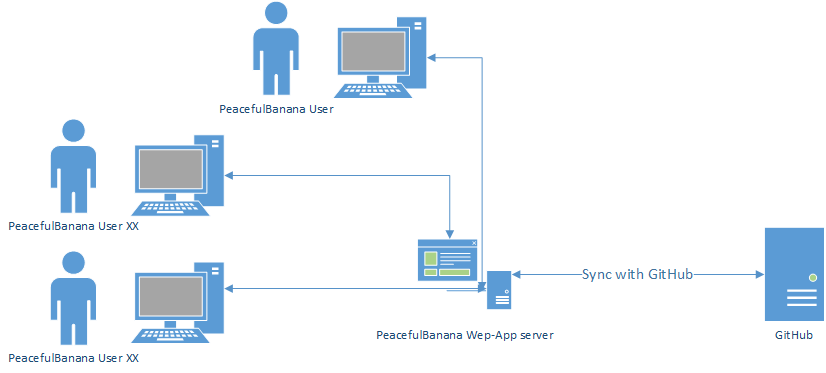
\includegraphics[width=\textwidth]{Clientservergithub}
    \caption{Overview of system design.}
    \label{ClientServerGithub}
\end{figure}

\section{Technology}
When choosing a framework for the prototype, several alternatives like Spring\footnote{\url{http://www.springsource.org/}}, WebObjects\footnote{\url{htpp://www.apple.com/webobjects/}} and Play Framework\footnote{\url{http://www.playframework.com/}} where discussed. Their architecture and our familiarity to the framework was a vital part of the selection. Based on these criteria the server was implemented with Grails a framework for web applications, it is better described in the section following.

\subsubsection{GitHub API}
\label{githubapi}
GitHub provides developers with the opportunity to use an API\footnote{Application programming interface} which gives them the possibility to communicate with GitHub and retrieve data directly from their database.  

When retrieving data from GitHub we used the provided API as described by their developer-site\footnote{\url{http://developer.github.com/v3/}}, this enabled us to control the sequence of data and when to ask for what type of data. All communication to GitHub servers are asynchronous and while therefore not introduce any performance related issues. 
 
\subsubsection{Grails}
Grails is an open source web application framework which uses the programming language Groovy(which is built on top of the Java Virtual Machine). When Grails was developed, it's developers aimed to re-use proven technologies such as Hibernate, Spring etc. 

\begin{figure}[H]
\centering
    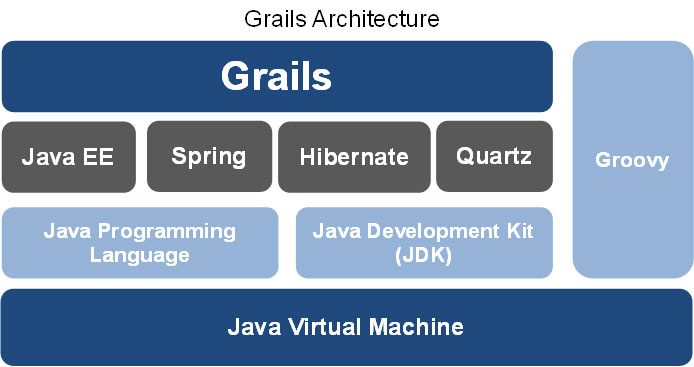
\includegraphics[width=0.8\textwidth]{Grails-Architecture}
\caption{Overview of Grails architecture.}
\end{figure}

Architectural grails is designed with the MVC\footnote{Model View Controller} pattern as a basis, this will expose the model\footnote{Data stored about the object.} in the view\footnote{With the restrictions on what data is viewable for the user.} and any manipulations to the model is done through a controller which controls that the data is correct input to the fields and what fields can be manipulated. An overview of the paradigm can be viewed in figure \ref{mvc-paradigm} below.

This pattern makes it easy for the developer to remain in control when creating a user interface and will ensure that the user can not manipulate fields without going through the controller\citep{reenskaug2009dci}. Using MVC increases flexibility and re-use by decoupling the user interface from the model and controller parts. The content of the view must reflect the state of the model, meaning when the model changes it notifies the view, which in turns updates itself. 
\begin{figure}[H]
    \centering
        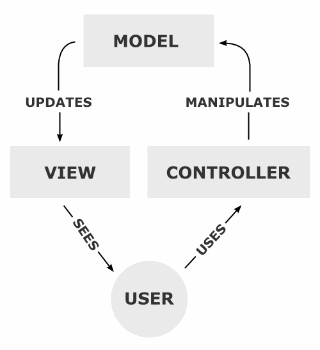
\includegraphics[width=0.6\textwidth]{MVC}
    \caption{Model-view-controller paradigm}
    \label{mvc-paradigm}
\end{figure}

\subsubsection{jQuery}
It was initially released under the MIT license in 2006 to make it easier to select DOM\footnote{Document-Object-Model} objects and create powerful dynamic web pages and applications.

JQuery has been used for AJAX\footnote{Asynchronous JavaScript and XML}, this is a way to change the contents DOM objects asynchronous from JavaScript.

\subsubsection{AwesomeCloud}
Awesome cloud is a plugin for jQuery for creating a tag cloud, it retrieves data from DOM-objects and rendered them as a cloud where the font-size increases with the occurrence of tags, the tag cloud is then drawn on the HTML5 canvas.

\subsection{Server and Database}
\label{sec:database}
During development we ran the application on a H2\footnote{\url{http://www.h2database.com/}} in-memory database. However the need for persistent storage arose, so we migrated to a MySQL database in order for the data to stay unchanged when we had to roll out updates to the tool. This choice was essential for the tool to function as described in the requirements, but the H2 database was more convenient and faster to debug during development.
\subsubsection{MySQL}
MySQL\footnote{MySQL: \url{http://www.mysql.com/}} is the world's largest open source relational database management system and can be used for a variety of applications. It is most commonly used with Web applications and works very well with dynamic web-pages, meaning that the content of each page is generated based on data loaded from a database as the page loads.

\subsubsection{Database description}
The PeacefulBanana GitHub specific domain-classes can be seen in Figure \ref{GithubDomainClasses}, and shows the relationship between the different data retrieved through the GitHub API.
All \emph{User specific} domain-classes can be seen in Figure \ref{UsersDomainClasses}.
A detailed walkthrough with data type categorization and description can be seen in Appendix \ref{app:database}
\begin{figure}[H]
    \centering
        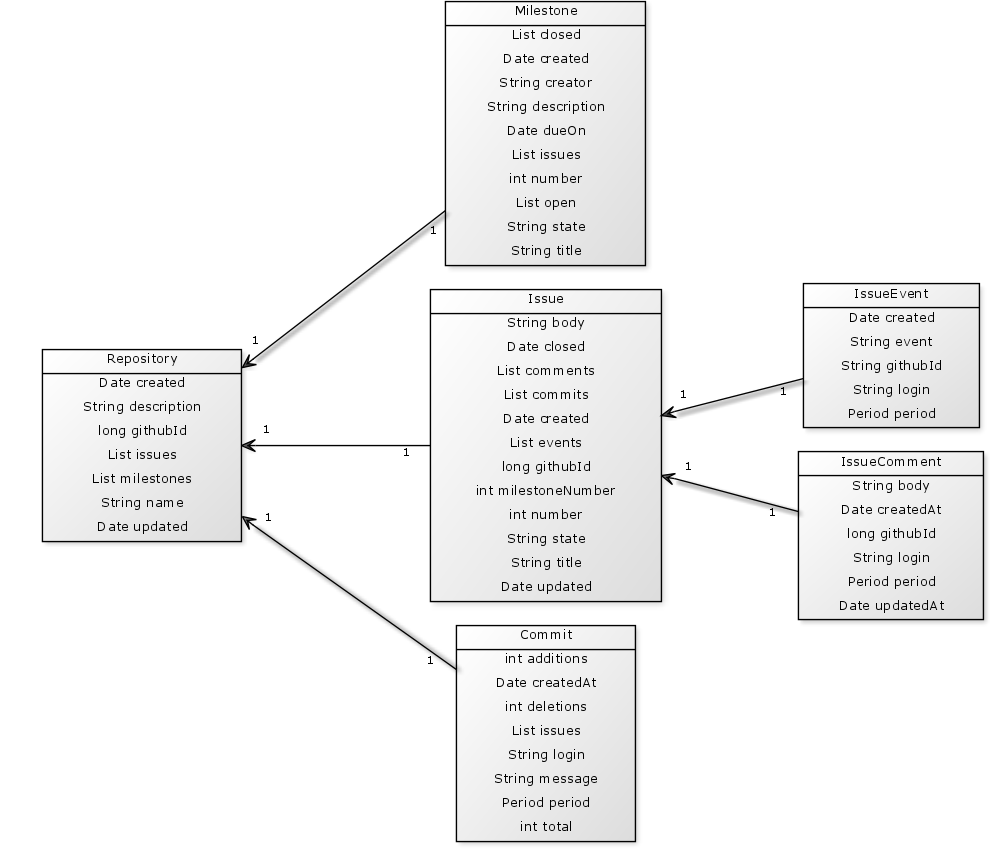
\includegraphics[width=\textwidth]{GithubDomainClasses}
    \caption{GitHub domain classes}
    \label{GithubDomainClasses}
\end{figure}
\begin{figure}[H]
    \centering
        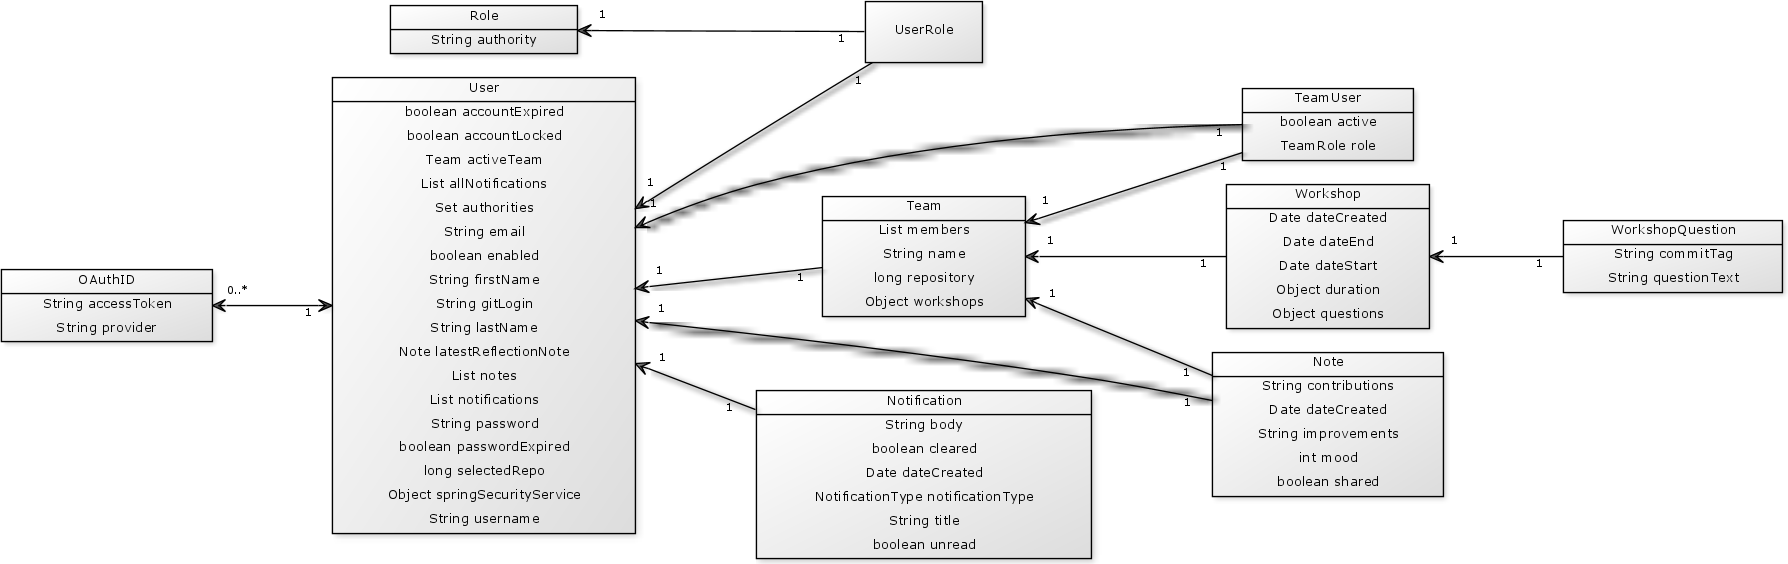
\includegraphics[width=\textwidth]{UsersDomainClasses}
    \caption{User domain classes}
    \label{UsersDomainClasses}
\end{figure}

\subsection{MIRROR CSRL}
This section describes the rationale behind the most important functionality implemented to PeacefulBanana, with relation to the Mirror CSRL cycle model. The section ends with a more detailed rationale behind the core functionality implemented. As described in Section \ref{mirrorsection} , the MIRROR CSRL model has four stages: 
\begin{enumerate}
    \item Plan and do work
    \item Initiate Reflection
    \item Conduct Reflection session
    \item Apply Outcome
\end{enumerate}
In this thesis, our research mostly focuses on the first two stages of the model, since PeacefulBanana is primarily to be used during work and as preparation for retrospective sessions. PeacefulBanana additionally includes some implementations focused towards the third stage \emph{Conduct reflection session}, as it also can be used during the session. 

\subsection{Plan and do work}
Figure \ref{plananddoworktable} shows functionality we implemented towards the \emph{Plan and do work} stage, and how our application help user(s) plan and perform their daily work tasks. 
Functionality in this stage is connected to \textbf{Sub research question 1}, which is focused on answering how the data collected from GitHub can be scaffolded in order to promote reflection. By carefully examining what GitHub offers itself, we could identify what they didn't offer and implement this functionality provided it could have a positive effect for promoting reflection for users. The challenge was not only to identify what data to collect, but also scaffold the collected data and present them to the users in a way that triggers reflection. \\
Adding mood to the \emph{Daily Reflection Note} implementation gave us the opportunity to create a mood-graph based on the team user's mood every day. This representation allows for a quick and easy mood comparison, which may encourage user's to look into why their mood differs opposed to the team's in a certain period of time. Such a discussion might occur at any time, either because a user browses on his own and wants to discuss his findings, or the team browses it together.  
The rationale of adding notifications to the application was made in order to give users context-relevant feedback and remind them of the daily reflection notes. \\
This functionality is also connected to \textbf{Sub research question 2}, which focuses on how to improve the tendency to reflect, both individually and in teams. 
\begin{figure}[H]
\centering
    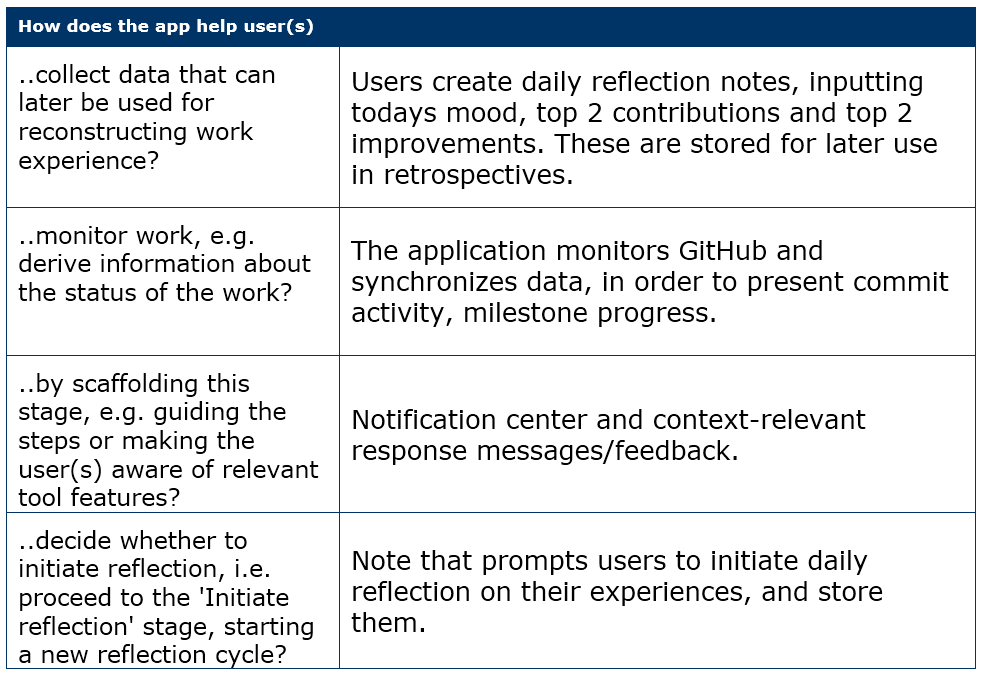
\includegraphics[width=\textwidth]{plananddoworktable}
\caption{Mirror CSRL Cycle - Plan and do work functionality \& implementations}
\label{plananddoworktable}
\end{figure}

\subsection{Initiate Reflection}
Figure \ref{initiatereflectiontable} shows functionality we implemented towards the \emph{Initiate Reflection} stage, and how our application help user(s) initiate reflection. Functionality in this stage is also coupled with \textbf{Sub research question 2}. The \emph{Reflection Workshop} functionality is implemented in order for teams to create a frame for their retrospective session. When a workshop has been added, individuals can also prepare by themselves by comparing their own data with the teams, i.e. the personal tag-cloud vs team tag-cloud and the mood-graph.  
\begin{figure}[H]
\centering
    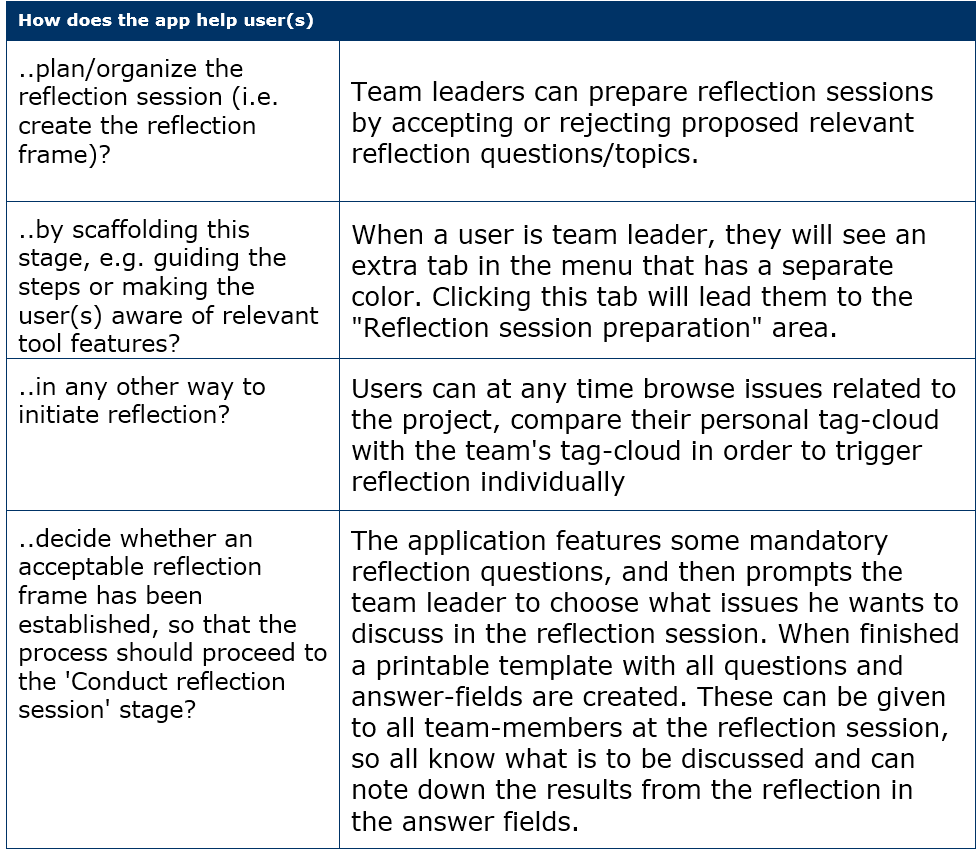
\includegraphics[width=\textwidth]{initiatereflectiontable}
\caption{Mirror CSRL Cycle - Initiate Reflection functionality \& implementations}
\label{initiatereflectiontable}
\end{figure}

\subsection{Conduct Reflection Session}
Figure \ref{conductreflectiontable} shows the functionality we implemented towards the \emph{Conduct Reflection Session} stage, and how our application help user(s) perform their retrospectives. 
This stage is not something we focused on, since most of the use of PeacefulBanana is doing daily work and using those data to prepare for retrospectives. Still the most notable functionality that is connected to this stage, is the ability to share and inspect reflection notes, meaning that teams can during reflection sessions wish to compare shared notes and create a discussion around these. Similarly teams can inspect repository data, like milestones and issues, and also tag-clouds connected to these. These tag-clouds can identify active issues which the team wishes to discuss during the retrospective. 
\begin{figure}[H]
\centering
    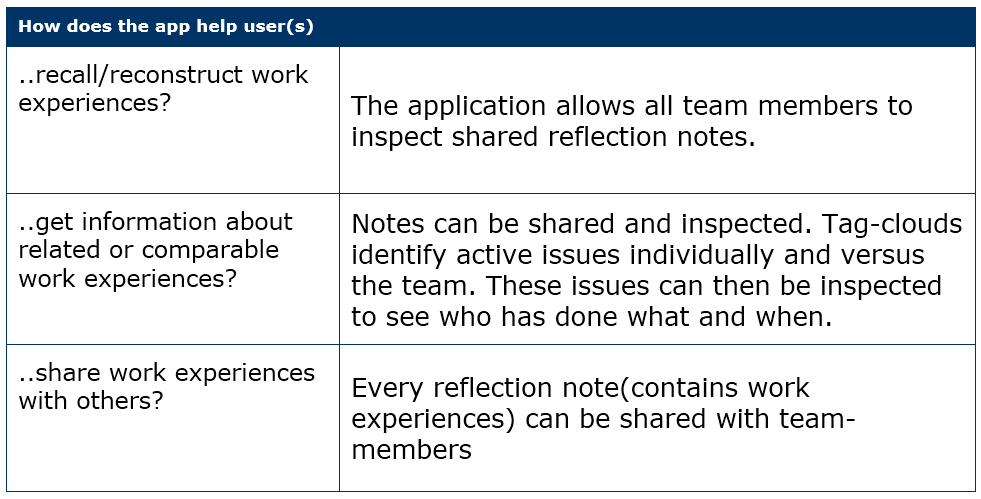
\includegraphics[width=\textwidth]{conductreflectiontable}
\caption{Mirror CSRL Cycle - Conduct reflection session functionality \& implementations}
\label{conductreflectiontable}
\end{figure}

\subsection{Core Functionality}
This section will describe the core functionality in the PeacefulBanana application. 
\paragraph{Daily reflection note}\mbox{}\\
Scaffolding is the act of creating a skeleton or a frame for the work to be done.
PeacefulBanana provides users with the ability to create reflection notes, where they reflect on that day's work and store it for later use. In this context the scaffolding is creating a frame for the reflection to be done, which includes text input and guiding questions. An example of such a reflection note can be seen in Figure \ref{dailynotefunc}. \\
In order to encourage users to reflect on their daily work and to avoid generic or non-constructive input, we connected questions to each input field, to act as guidance. For each input, the application provides a question, like \emph{How did you feel about todays work?} for the mood input. Adding these questions helps users think back on their experiences that day and perform a reflection on these. 
\begin{figure}[H]
    \centering
        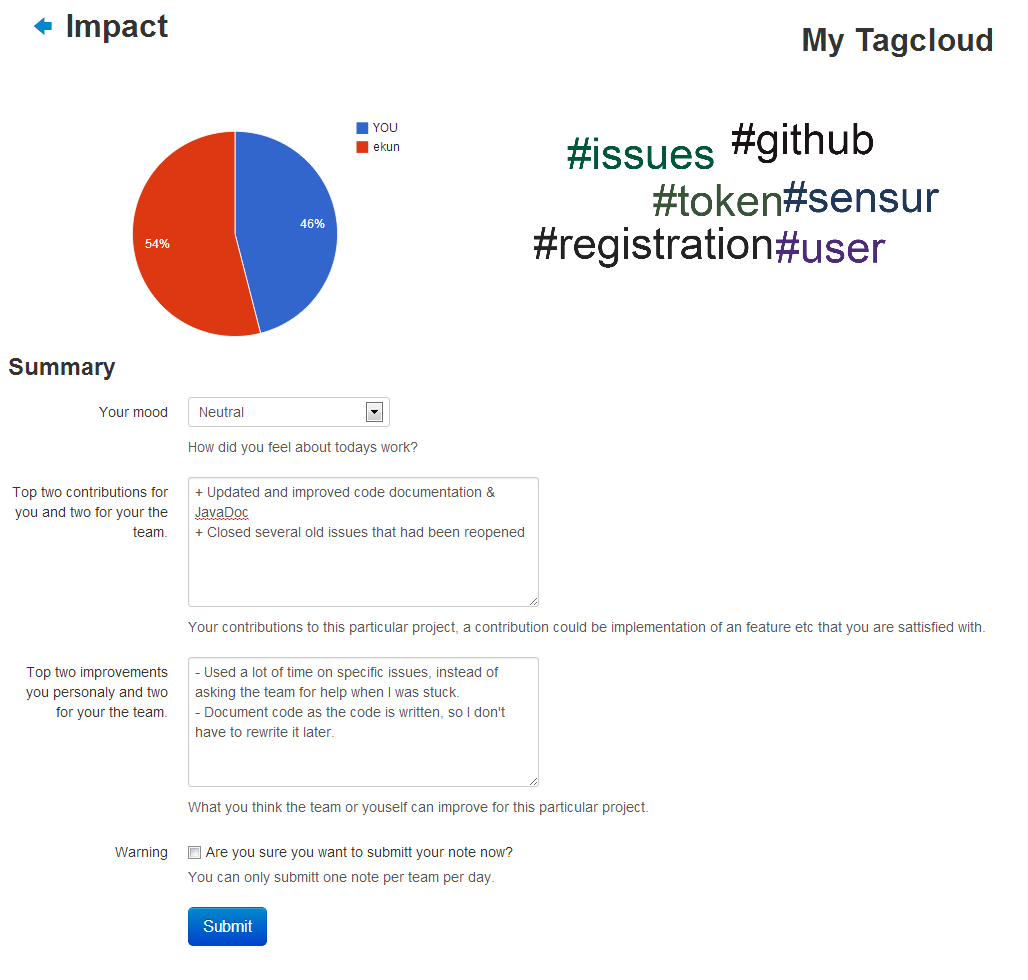
\includegraphics[width=\textwidth]{dailynote}
    \caption{PeacefulBanana reflection note}
    \label{dailynotefunc}
\end{figure}

\paragraph{Mood graphs}\mbox{}\\
When creating a reflection note, users can connect their current mood, that is how they felt, to the reflection note. By adding the ability to connect mood to notes each day, the tool can present meaningful mood-averages back to the users. These mood averages are used by PeacefulBanana to generate a mood-graph, depicting a user's or a team's mood over a period of time. 
By presenting this shared team-average mood, user's get an indication of how the work is perceived by the other group members and the team can create a discussion around certain trends in mood, or even why certain users stand out from the rest of the team's mood. 
An example of such a mood graph can be seen in Figure: \ref{moodgraphfunc}
\begin{figure}[H]
    \centering
        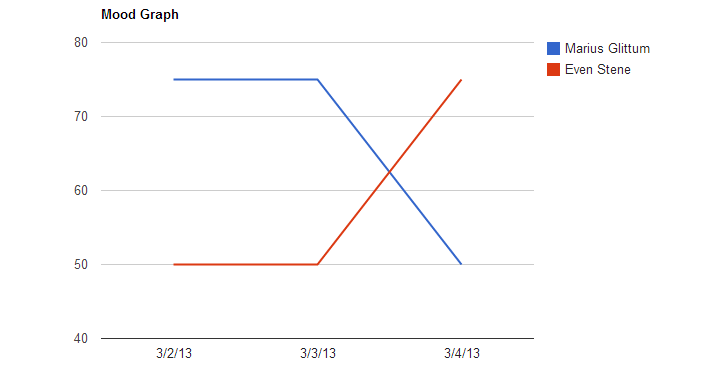
\includegraphics[width=\textwidth]{moodgraph}
    \caption{PeacefulBanana Team Mood-graph}
    \label{moodgraphfunc}
\end{figure}
\paragraph{Tag-clouds}\mbox{}\\
PeacefulBanana also provides the user with individual and team-wide tag-clouds. These tag-clouds are based on the user's or the team's activity in a GitHub project over a period of time. The tag-cloud elements are weighted according to how much the particular \emph{\#tag} has been worked with, the more activity the bigger the word. Implementation of the tag-clouds allows user's to see trending events in their own activity trajectory, but also compare it with the rest of the team. This enables the user to see how their work is affecting the team's work, but also gives the team an indication on what has been worked with over different periods of time(i.e. a development iteration). 
\begin{figure}[H]
    \centering
        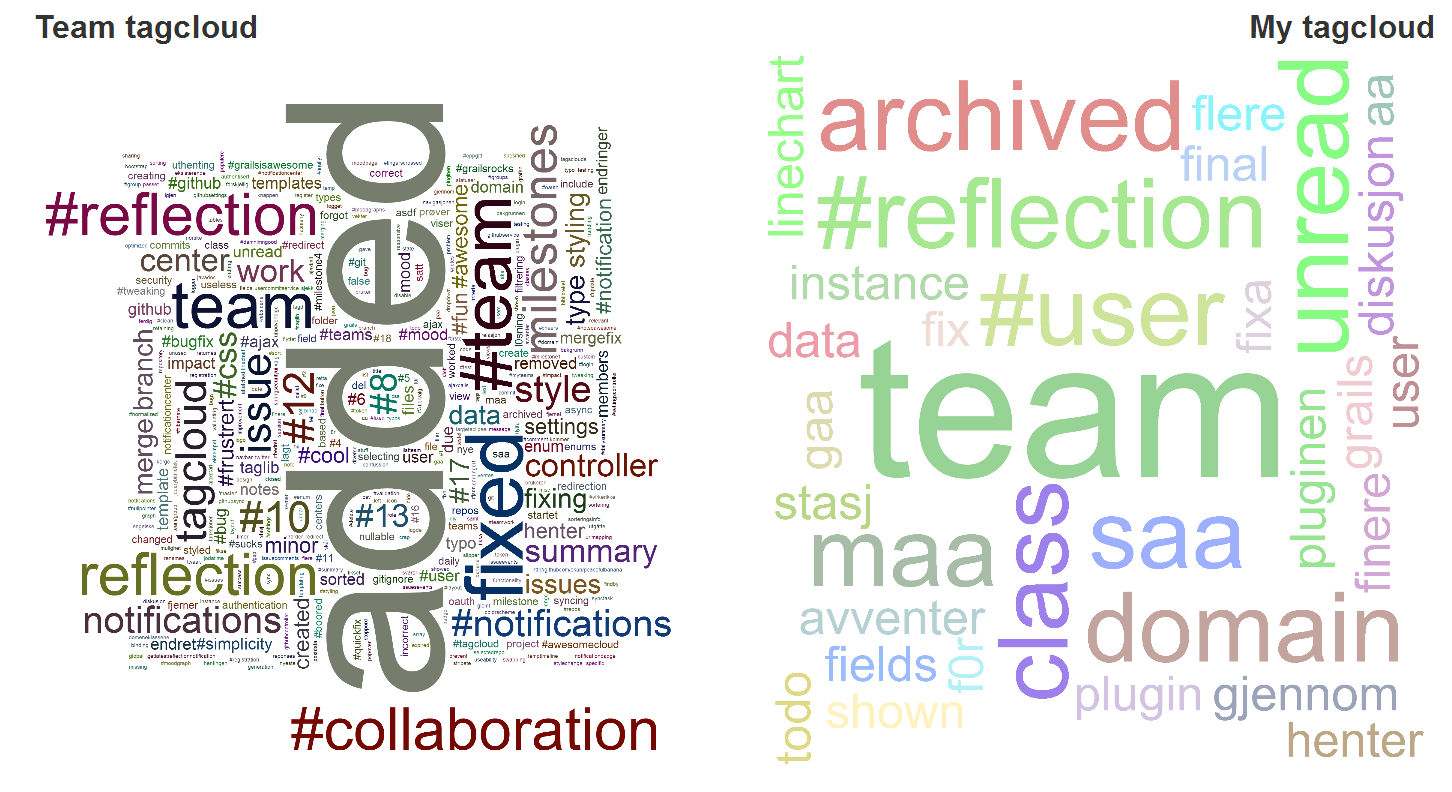
\includegraphics[width=\textwidth]{tagcloud_teamvsmy}
    \caption{PeacefulBanana tag-cloud implementation}
    \label{tagcloudfunc}
\end{figure}

\paragraph{Sharing of data}\mbox{}\\
Reflection notes can be shared with a user's team, should they want to.  PeacefulBanana collects team-relevant data from GitHub , scaffolds and presents these to users. This data gives the team the ability to see who is working on what, are there any trending issues in the team that can be intercepted and solved and more.  
Figure \ref{MyNotes} shows how PeacefulBanana user's can see their notes and the notes' creation date, owning user, what team that user is on and the share status of the note. The user can also simply filter between their own notes or shared notes by their current team. This is shown in Figure \ref{notes_shared}
\begin{figure}[H]
    \centering
        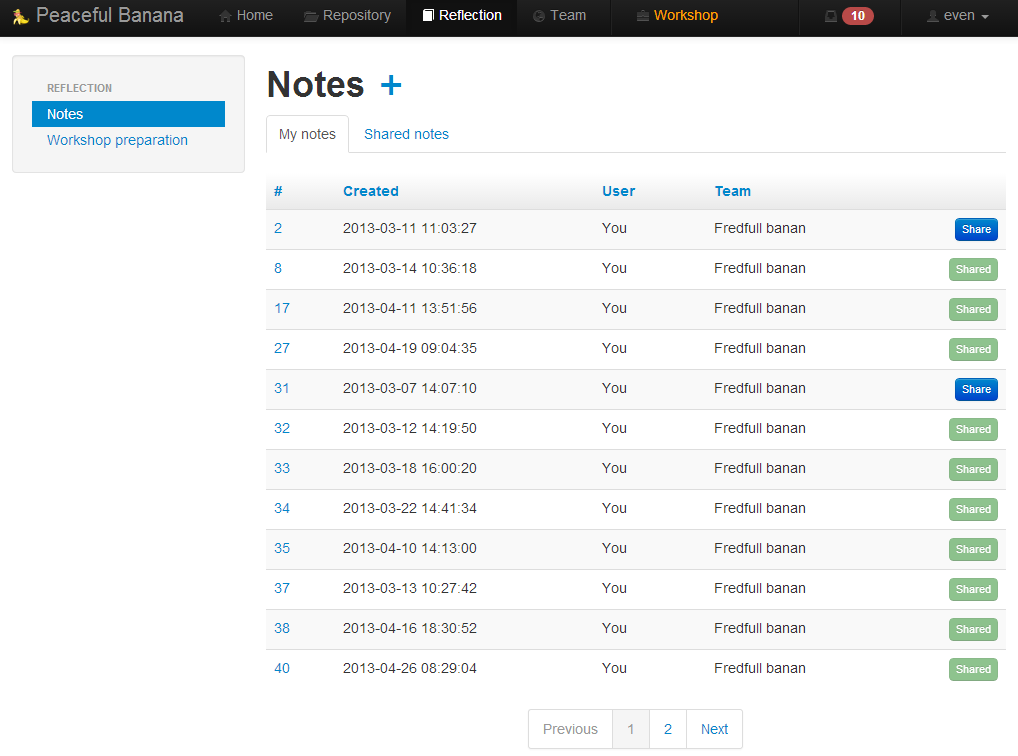
\includegraphics[width=\textwidth]{MyNotes}
    \caption{PeacefulBanana user notes}
    \label{MyNotesFunc}
\end{figure}
\begin{figure}[H]
    \centering
        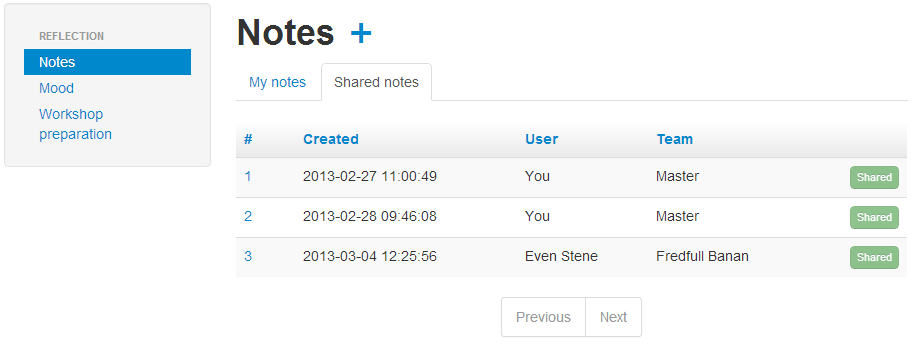
\includegraphics[width=\textwidth]{notes_shared}
    \caption{PeacefulBanana shared team notes}
    \label{notes_sharedfunc}
\end{figure}

\subsubsection{Repository}
In addition to functionality related to the \emph{Daily Reflection Note} and team retrospective sessions, we also implemented functionality aimed towards individual and collaborative reflection outside of these frames. This includes gaining an overview of the current project, the status of milestones and related issues. The rationale for implementing these functionalities is that we want to keep the required use of PeacefulBanana to a minimum, therefore only the 5-minute daily reflection is required to gain advantages towards the retrospective session. However, if a user or the whole team wants to dive deeper into the project data, they can do so in the \emph{Repository} section. Here users can see the teams commit activity, see the status of milestones and filter them based on this status. Clicking on a specific milestone will show all issues connected to the milestone and a tag-cloud containing that milestone's most used tags. Figure \ref{milestonefunc} shows an example of such a milestone with related issues, and Figure \ref{tagcloudfunc} shows the tag-cloud connected to this milestone. \\
This means users or teams can identify certain issues that dominate, and can easily inspect these by clicking on them. Inspecting an issue will present comments, commit references and events concerning that issue. This enables individuals to inspect and revisit experiences, and allows teams to create a discussion around issues or milestones outside of the retrospective sessions. 

\begin{figure}[H]
    \centering
        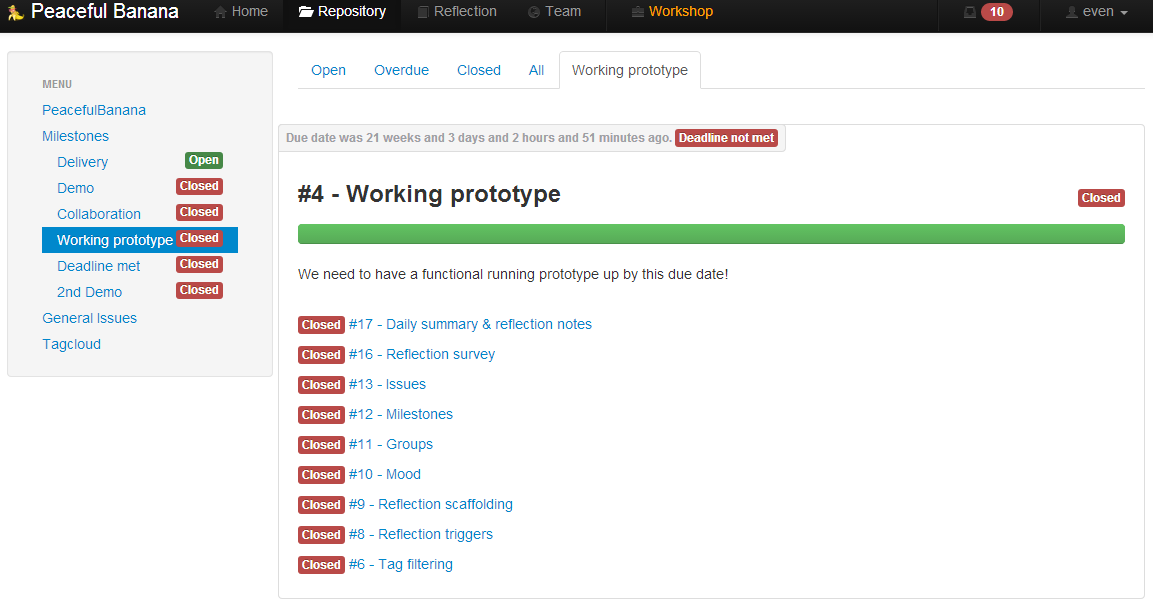
\includegraphics[width=\textwidth]{milestonefunc}
    \caption{PeacefulBanana - Repository milestone and issues}
    \label{milestonefunc}
\end{figure}

\begin{figure}[H]
    \centering
        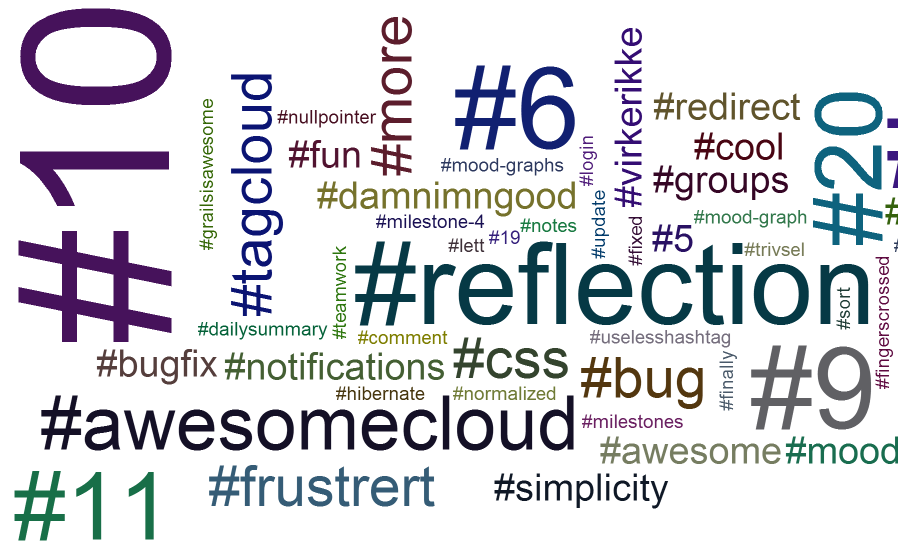
\includegraphics[width=\textwidth]{tagcloudfunc}
    \caption{PeacefulBanana - Repository milestone tag-cloud}
    \label{tagcloudfunc}
\end{figure}

\subsubsection{Reflection sessions}
One of the primary functionalities we implemented, in addition to the daily reflection note, was the \emph{Reflection Workshop}. The manager of each team will see a separate \emph{Workshop} tab. The workshop area allows managers to prepare for retrospective sessions, by creating a workshop for that period of time(i.e. an iteration that have lasted for the last two weeks). Figure \ref{picher} shows an example of such a workshop. \\ 
When the workshop has been created, users are met with three accordion headers\footnote{An accordion is a collapsible content panel for presenting information in a limited amount of space}. The accordions contain some mandatory questions which is some general reflection questions that is relevant to discuss in retrospective sessions, and so these cannot be removed from the workshop. The PeacefulBanana application also uses gathered data about the most used tags, to generate some proposed questions. The rationale behind this choice is that if the team has had a high activity with a certain tag, it is a high possibility that it's also important to discuss. Examples of these generated questions can be seen in Figure \ref{ref}. Ultimately though, it is the manager of the team that chooses what questions or tags that should be discussed in the retrospective session. Therefore if the manager feels that one or more of the generated questions are unimportant, they can be removed. \\
Finally the manager can browse a list of all tags, with the most active at the top, and simply click the tag that should be discussed as part of the retrospective session. If a tag is clicked under the \emph{Possible tags questions} they will be instantly moved to the \emph{Questions generated} section, and vice-versa deleted questions will be moved to the list of possible tag questions. Figure \ref{bilde} shows how the tag list is presented in the application. 

\begin{figure}[H]
    \centering
        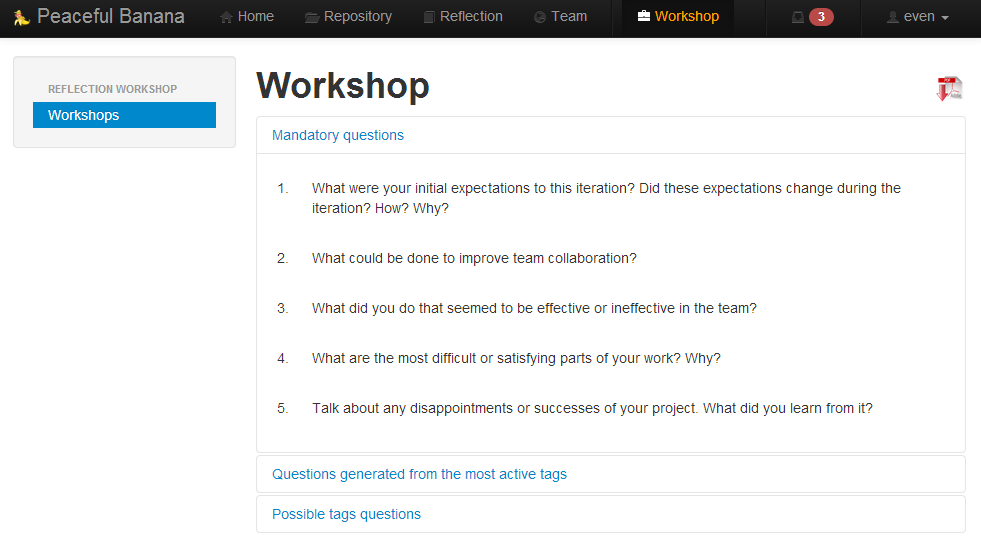
\includegraphics[width=\textwidth]{workshopmandatory}
    \caption{PeacefulBanana Workshop - Mandatory questions}
    \label{workshopmandatoryfunc}
\end{figure}
\begin{figure}[H]
    \centering
        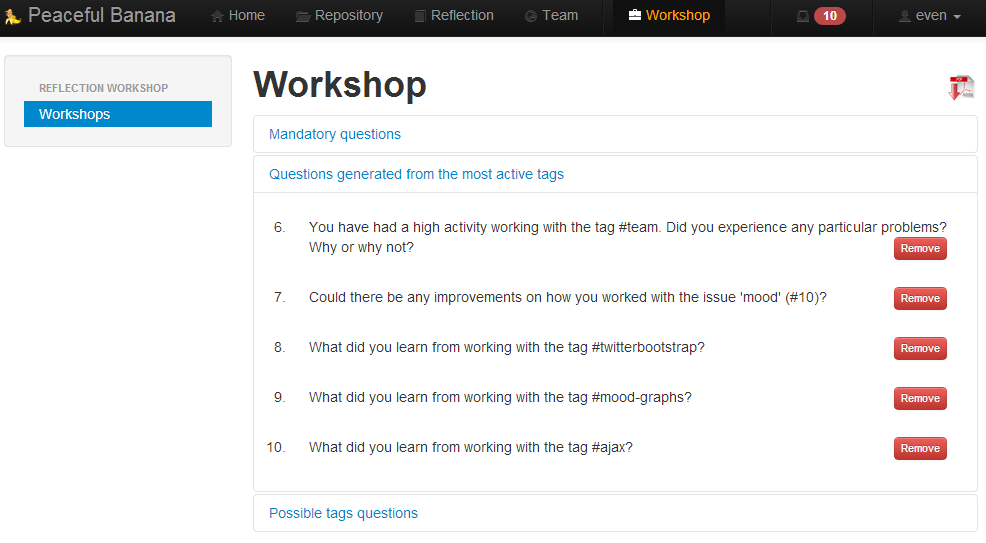
\includegraphics[width=\textwidth]{workshopgenerated}
    \caption{PeacefulBanana Workshop - Generated questions based on active tags}
    \label{workshopgeneratedfunc}
\end{figure}
\begin{figure}[H]
    \centering
        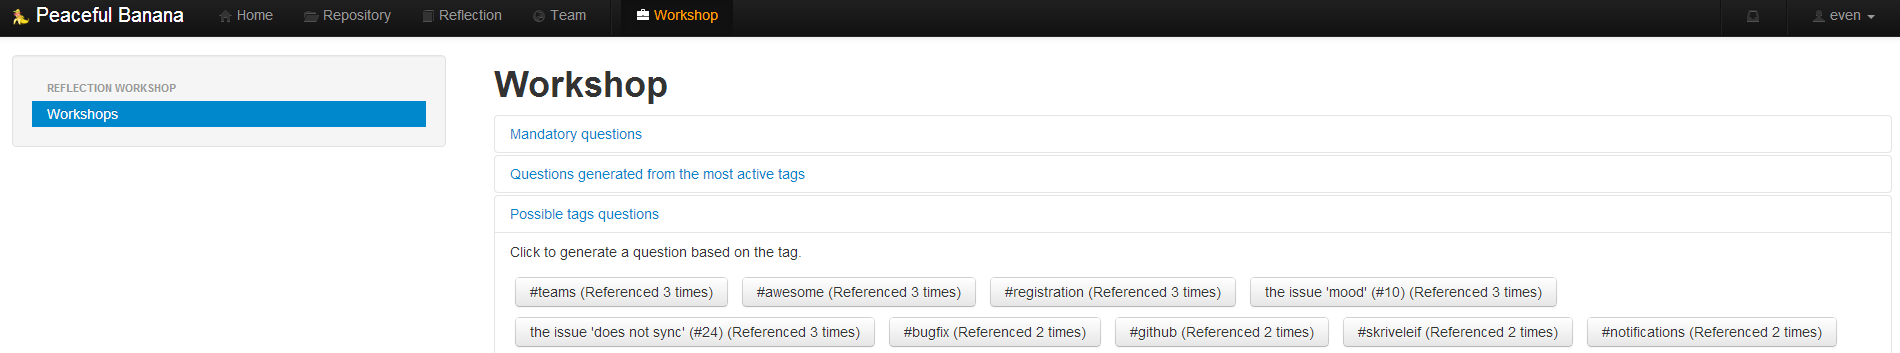
\includegraphics[width=\textwidth]{workshoppossible}
    \caption{PeacefulBanana Workshop - Possible questions based on tags}
    \label{workshoppossiblefunc}
\end{figure}
